\section{Design}

The system we designed and implemented consists of three components: the OT
algorithm, the server, and the client. We implemented a centralized model where
clients don't talk to each other but rely on the server for coordination. The
clients generate operations based on the local information and submit it to the
server. The server reconciles operations from different clients, resolves any
conflicts, and broadcasts the results to all clients. Finally, each client
updates their local state in accordance with the information received from the
server. The OT algorithm is involved in each of the steps above and is therefore
the core of our system. Now let's take a look at each component in more detail.

\subsection{OT Algorithm}
\label{sec:design_alg}

At a high level, our operational transformation (OT) framework ensures that all
clients and servers agree on a total order in which operations are applied. We
achieve this by making each client operation in one of the three possible
states: {\em committed}, {\em pending}, and {\em unsent} (we'll explain them in
more detail in Section~\ref{sec:design_client}). Only committed operations are
treated as ``hard truth'' by the servers and clients, and clients only receive
committed operations from servers. Both pending and unsent messages will also be
referred to as {\em uncommitted} messages for the rest of this document.

Each operation alone must contain enough information to express its intention,
and conflict resolution is performed using this information. We achieve this by
assigning each operation a version number it operates on, so that the intention
of the operation can be extracted even if messages arrive in different order.
Every operation, when committed, will be applied to states (called {\em
committed states}) of the clients and the servers, and will advance the version
number by one. We only advance the version number when an operation is committed
so that version numbers are kept consistent across all participants, i.e. the
same version number from different clients is guaranteed to refer to the same
historical version of the document.

A key feature of our OT algorithm is that the version numbers as well as other
information associated with uncommitted operations are subject to change. After
the server receives an operation, it will apply the server-side policy to merge
this operation into the document's edit history, preserving the arriving
operation's intention, and finally transform the operation into a committed
operation and broadcast it to all clients. The clients receive committed
operations from the server and apply them in order. This rigorous version
management scheme ensures that all servers and clients agree on a single order
of all committed operations. In principle it is enough to ensure the correctness
of the system because only committed operations are treated as ``hard truth''
(which means they can overwrite uncommitted operations if necessary).
Figure~\ref{fig:walkthrough} shows an example work flow to illustrate how the
algorithm works.

\begin{figure}[t!]
  \centering
  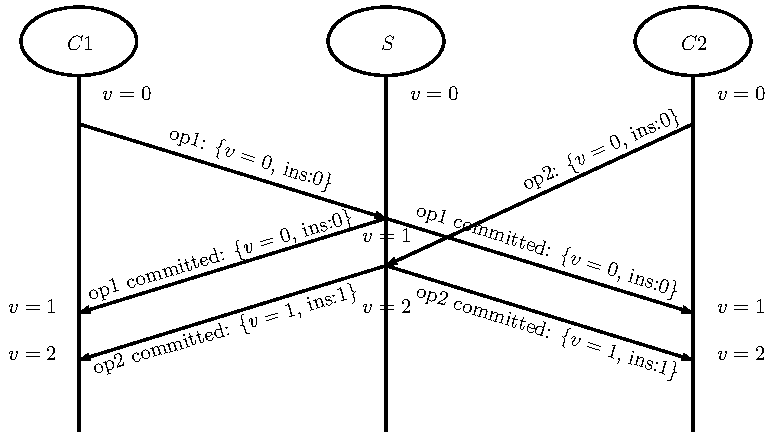
\includegraphics[width=0.45\textwidth]{walkthrough.pdf}

  \caption{An example work flow of the system. $C1$ and $C2$ are two clients,
  and $S$ represents the server. Note that the server resolves conflicting
  operations (op1 and op2) submitted by the two clients when op2 reaches the
  server, and op2 is transformed to be operate on version 1 instead of version
  0. The insertion position of op2 is also pushed back by one when committed.
  The Clients and the server all settle with the same version (version 2) at the
  end of the process.}
  
  \label{fig:walkthrough}
\end{figure}

\subsection{Server}
\label{sec:design_server}

As mentioned in Section~\ref{sec:design_alg}, all conflict resolutions take
place on the server side. For simplicity reasons we only implemented
single-character operations to minimize the complexity of conflict resolution.
The server also stores the entire edit history (a sequence of all committed
operations) so that it can resolve conflicts for out-of-date operations
(operations that refer to older version numbers).

Whenever the server receives an operation from one of the clients, it first
checks if the operation operates on the most current document version. The
server can safely apply the operation and mark it as ``committed'' if the
operation is intended to modify the most current version of the document.
Conflict arises if an incoming operation requests modification to the document
based on an older version. When this happens, the server finds the position the
incoming operation refers to in the document edit history, and iteratively
resolves conflict between the incoming operation and every committed operation
after this position. After each round of conflict resolution, the incoming
operation's version number (referring to the document version it operates on)
will be incremented; therefore after the entire conflict resolution process
ends, the incoming operation's version number will become the most current
version, and we say that the server has effectively ``transformed'' the incoming
operation to a committed operation, and can thus safely apply it and broadcast
it to all clients.

We omit the details about the pairwise conflict resolution policy because it is
relatively straightforward in our single-character use case. The basic idea is
to keep track of the intentions of two conflicting operations. For example, an
{\tt Insert} to a position before a {\tt Delete} should push forward the
position that {\tt Delete} operates on by one, and two {\tt Delete}s to the same
position in the same version should only be done once. Many other policies may
also result in a usable system.

It is worth noting that we don't impose any constraints on the conflict
resolution policy for consistency requirements. Our operational transformation
framework does not rely on the commutativity of conflict resolution to function
correctly.

\subsection{Client}
\label{sec:design_client}

The client side of the system has the most complex program logic in our system,
because it needs to handle both committed and uncommitted states. We need to
account for uncommitted state because the application shouldn't block (prevent
the user from typing additional characters) while waiting for response from the
server. Due to network delay and/or message loss, a client's local state is
usually ahead of the server's, and different clients' states may easily diverge.
Now we describe how we address these problems.

First of all, a client is only allowed to have one {\em pending} operation at a
time. An operation is said to be in {\em pending} state if the client has
already sent it to the server, but the server hasn't sent it back (via
broadcast, actually, because other clients also need this information) in its
committed form. Enforcing this policy is reasonable because we want strong
sequential consistency for operations performed by the same client.

Once a client generates an operation and sends it to the server, it has an
operation pending and therefore cannot send more operations to the server before
it hears back from the server again. However, the client should not be blocked
from generating new operations during this time interval. All operations
generated by a client after the pending operation are set to the {\em unsent}
state, and they refer to {\em tentative} version numbers based on the client's
best knowledge. Once the pending operation is confirmed by the server, the
client will examine the version number of the committed operation and update
tentative version numbers in unsent operations accordingly, before sending the
next operation (the first one in the unsent queue) to the server.

In the process mentioned above, if the client receives from the server a
committed operation initiated by another client, the client side program should
also update tentative version numbers in unsent operations accordingly. In
summary, tentative version numbers are obtained by adding committed version
numbers (which are ``hard truths'') to the client's ``guess'' of how the
committed version number may change after the pending operation ``returns''. A
decent guess for the client to make is always to assume that there are no other
clients editing at the same time, so the committed version should be incremented
by one by the time the pending one returns. If some other committed operation
arrives before the client's own pending operation returns, then there must have
been some other guy changing the document at the same time, and her change made
it to the server first. The client therefore should observe this effect and
adjust its ``guess'' accordingly by ``rebasing'' all tentative version numbers.
The only difference in this case is that the client now cannot send a new
operation to the server, because its pending operation hasn't ``returned'' yet.

Every time upon receipt of a committed operation, the client applies it to the
committed state, merges the new committed state with uncommitted operations, and
presents the result to the user. We do assume that committed operations always
arrive in order. Many widely used technologies, such as TCP~\cite{tcp} or higher
level protocols based on TCP, provide this guarantee.
